\documentclass[11pt]{article}

\usepackage{amssymb, amsmath, amsthm}
\usepackage{graphicx} 
\usepackage{wrapfig}
\usepackage{mathtools}
\DeclarePairedDelimiter\floor{\lfloor}{\rfloor}

\title{ Homework 2 }
\author{ Jacob Hurst }
\date{\today}

\begin{document}

\maketitle
\clearpage

\section{Question 1}
\subsection{We know that, among trees of depth d, the largest one is the perfect tree, which has $ 2^{d+1} - 1 $ nodes. This is an AVL tree, so we know the biggest an AVL tree of depth $ d $ can be. Prove that the smallest AVL tree of depth $ d $ has $ fib(n+3) - 1 $ nodes.  Include a diagram showing what they look like for $ d = 0 $ up to $ d = 4. $ }

Max AVL Tree: depth $d$, $2^{d+1}-1$ nodes. \\Min AVL Tree: depth $d$, $fib(d+3)-1$ nodes. \\Let $T_L$ be the height of the left subtree and $T_R$ be the height of the right subtree. \\The AVL balance property is the property that $T_L - T_R = -1, 0, $ or $ 1$. \\Considering these properties with respect to our AVL tree we can observe that $T_L = (d-1)$ and $T_R = (d-2)$ throughout our trees subtrees. \\If we let $Xd$ be the minimum number of nodes in our depth $d$ AVL tree, then we arrive at the following recurrence relation. \\$Xd = X(d-1) + X(d-2) + 1$ where $X(d-1)$ and $X(d-2)$ represent left and right subtrees and $1$ represents the current node. \\We would like to prove that $Xd = fib(d+3) - 1$.
\\
\\
Proof by Induction:\\
Base Cases: \\$X_0 = 1 = fib(0+3) - 1 = 1, X_1 = 2 = fib(1+3) - 1 = 2$\\
Inductive Hypothesis: \\Assume true for $Xd$ and $X(d-1)$.\\
Inductive Step: \\Show $X(d+1) = f(d+4) - 1$.\\
Begin:\\
$
X(d+1) = Xd + X(d-1) + 1 \\= (fib(d+3) - 1) + (fib((d-1)+3) - 1) + 1
$ (IH) $ \\= fib(d+3) + fib((d-1)+3) - 1 = fib((d+1)+3) - 1 $ (Fibonacci) $ = f(d+4) - 1 \qed.$ \\\\Illustration:

\begin{figure}
  \begin{flushleft}
    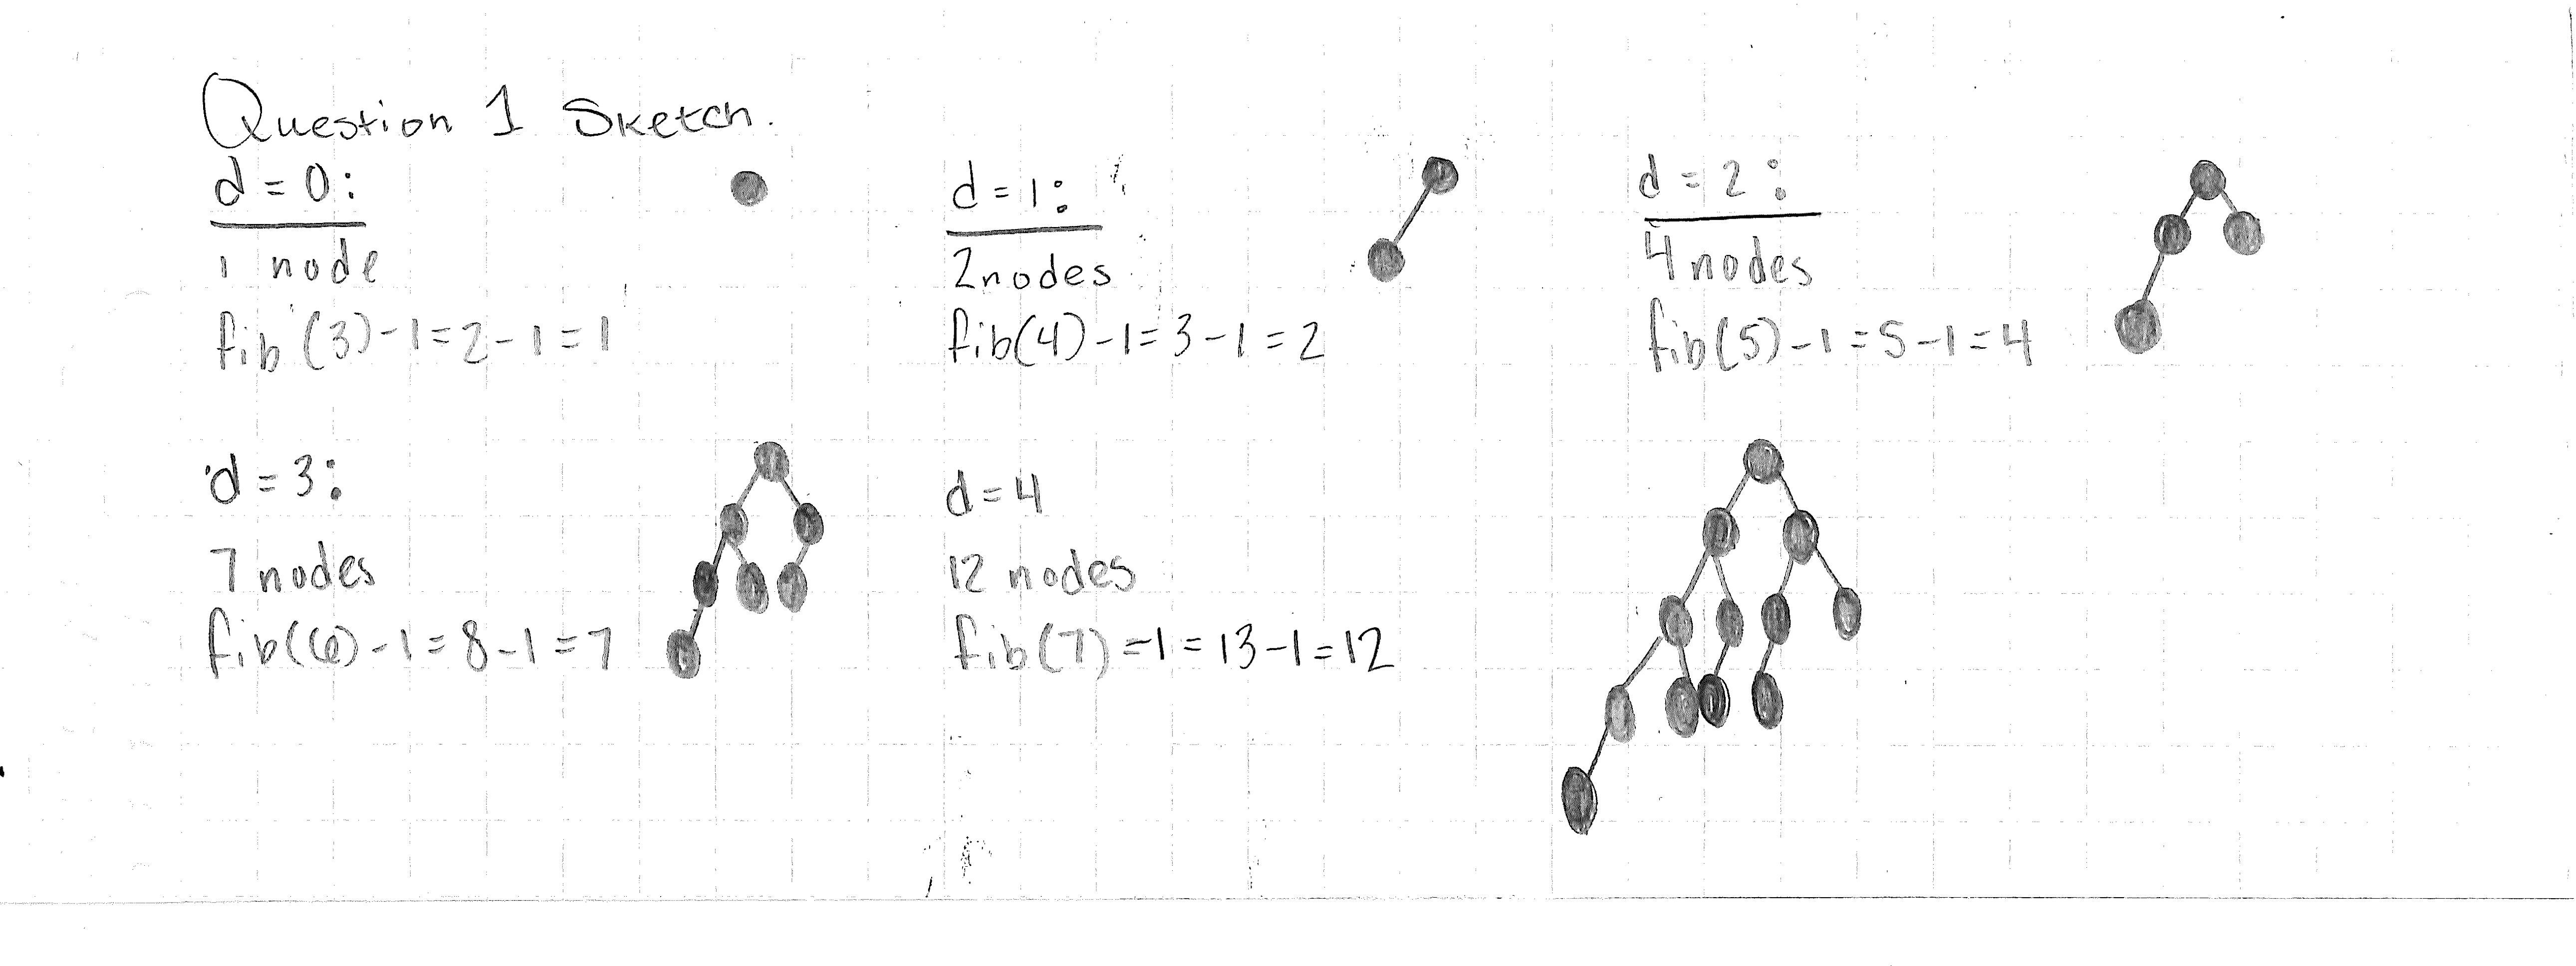
\includegraphics[width=1.5\textwidth]{q1.png}
  \end{flushleft}
  \caption{Diagram of AVL Trees, depth = 0, 1, 2, 3, 4.}
\end{figure}

\section{Question 2}
\subsection{A generalized Fibonacci sequence $ G(n) $ is defined by initial conditions $ G(0) = A, G(1) = B $, and the usual recurrence $ G(n) = G(n-1) + G(n-2) $ for $ n \geq 2 $.  It is called geometric if $ G(n) = C\phi^n$. There are three possible values for $ \phi $ in a geometric generalized Fibonacci sequence (GGFS). Find all three.}

From the usual recurrence, we have $ G(n+2) = G(n+1) + G(n) $. \\Plugging in $C\phi^n$ yields $ C\phi^{n+2} = C\phi^{n+1} + C\phi^n \rightarrow \phi^{n+2} = \phi^{n+1} + \phi^n \\\rightarrow \phi^2 = \phi + 1 \rightarrow \phi^2 - \phi - 1 = 0$. \\\\By the Quadratic Formula, we find $\phi = (1+\sqrt 5)/2 $ and $ \phi = (1-\sqrt 5)/2$ (Golden Ratio) as the first two solutions. The third solution is simply $\phi = 0$ as it satisfies the relation.

\section{Question 3}
\subsection{Show that every generalized Fibonacci sequence is a linear combination of two GGFS's, and therefore is of the form $ C\phi^n + D\psi^n$, where the bases $ \phi $ and $ \psi $ are two of the three values computed in problem 2. Since the growth rate of this function is controlled by the larger of $ \phi $ and $ \psi $ in absolute value, this gives a very precise estimate for the Fibonacci numbers. Use this to conclude that the maximum depth of an AVL tree on $ n $ nodes is $ Elog(n) $, where $ E $ is a constant.  Give $ E $ as an explicit formula, and also compute it to three decimal places using a calculator.}

Let $g(n-1) = C\phi^n$ and $g(n-2) = D\psi^n$, by the usual recurrence in question 2, we have that $g(n) = C\phi^n + D\psi^n$. \\Where $\phi = (1+\sqrt 5)/2 $ and $\psi = (1-\sqrt 5)/2$. We can use the initial conditions $n=0, n=1$ to find C and D.\\
\\$ n=0: C + D = 0 \rightarrow D = -C$
\\$ n=1: C\phi + D\psi = 1$. \\\\Plugging in $D = -C$ to the second initial condition result.
$ C\phi -C\psi = 1 \\\rightarrow C(\phi - \psi) = 1 \rightarrow C((1/2 + \sqrt 5/2) - (1/2 - \sqrt 5/2)) \rightarrow C\sqrt 5 = 1 \\\rightarrow C = 1/{\sqrt 5}$.\\\\So, we have $g(n) = 1/{\sqrt 5}\phi^n - 1/{\sqrt 5}\psi^n$. \\\\In terms of our AVL tree, this is $Xd = 1/{\sqrt 5}\phi^{d+3} - 1/{\sqrt 5}\psi^{d+3}$. \\Since the absolute value of $\phi \approx 1.6 $ and the absolute value of $\psi \approx 0.6$, we can approximate $Xd$ by $Xd \approx 1/{\sqrt 5}\phi^{d+3}$ and then solve for d to find the max depth. \\\\Taking $log_\phi$ of both sides yields $log_\phi(Xd) \approx (d+3) - log_\phi(\sqrt 5 )$. \\We convert this to $log_2$ by log rules and arrive at $d \approx log_2(Xd)/{log_2(\phi}) + log_2(\phi)$. \\\\We disregard the constants and focus on $d \approx log_2(Xd)/{log_2(\phi})$. $ E \approx 1.440$ or $E = 1/{log_2(\phi)} $.

\section{Question 4}
\subsection{Find the smallest possible Red-Black trees of heights up to 10. For the last few, rather than drawing every node, you may use the notation $ P_d $ to indicate a perfect subtree of depth $ d $.  Try to deduce a general formula for the number of nodes in the smallest Red-Black tree of height $ h $. Then, use big-O notation to write it as $ \theta(\xi^n) $ for some constant $ \xi $. As in problem 3, invert this formula to conclude that the maximum depth of a Red-Black tree on $ n $ nodes is $ Clog(n) $, where $ C $ is a constant.  Give $ C $ as an explicit formula, and also compute it to three decimal places using a calculator.}

As seen in the diagrams below, a minimal red-black tree with height h contains a path of alternating red and black nodes on its max depth path (which contains $n+1$ nodes). \\Equivalently, we can find that the longest path has $\floor*{h/2} + 1$ red nodes. Each of the right subtrees contain the necessary number of black nodes to balance the red-black tree (these are given by $2^n - 1$). \\From this, we can find that $n = 2^{\floor*{h/2}+2} + (h - 2^{\floor*{h/2}})-3 \\\rightarrow n = 2^{\floor*{h/2}+2} - 3 \\\rightarrow (n+3)/4 = 2^{\floor*{h/2}+2} $. \\Taking log of both sides to find h gives us $\floor*{h/2} = log_2(n+3) - log_2(4) \\\rightarrow \floor{h/2} = log_2(n+3) - 2 \\\rightarrow h/2 = log_2(n+3) - 1 \\\rightarrow h = 2(log_2(n+3) - 1)$ and by big-O notation $h = O(log_2(n))$ and $C = 2$.\\\\Alternatively, we can observe that a red-black tree is also a binary tree. The max is in a perfect binary tree is $ n = 2^{h+1}-1 \rightarrow h = log_2(n+1) - 1 \rightarrow h = O(log_2(n))$.\\\\Illustration:

\begin{figure}
  \begin{flushleft}
    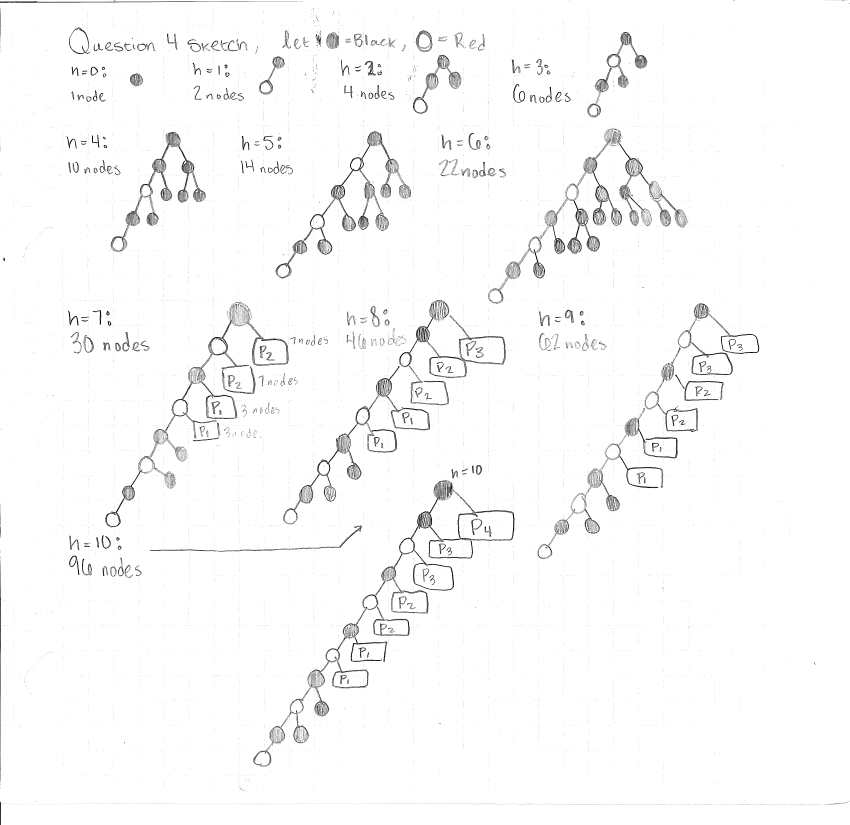
\includegraphics[width=1.5\textwidth]{q4.png}
  \end{flushleft}
  \caption{Diagram of h = 0 to h = 10 small red-black trees.}
\end{figure}

\end{document}  